\section{Empirical Results}\label{sec:results}

\section{Data}\label{subsec:data}
In the empirical analysis, we consider the risk reduction capability of the BTC-future (BTCF) on five cryptos
, BTC, ETH, ADA, LTC, and XRP, and five crypto indexes, BITX, BITW100, CRIX, BITW20, and BITW70,
For each of the 10 hedging portfolios, a crypto or index is considered as the spot and held in a unit size long position,
and the BTCF is held in short position of OHR unit in order to reduce the risk of the spot.
All the hedging portfolios are cross asset hedging except the BTCF portfolio.
ETH, ADA, LTC, and XRP are popular cryptos tradable in various exchanges and have large market capitalization.
BITX, BITW100, and CRIX are market-cap weighted crypto indexes with BTC as constituent.
BITX and BITW100 tracks the total return of the 10 and 100 cryptos with largest market-cap respectively.
CRIX decides the number of constituents by AIC and track that number of cryptos with largest market-cap.
In our case, the number of constituents in CRIX is 5.
BITW20 is also a market-cap weighted crypto index but with 20 largest market-cap cryptos outside the constituents of
BITX.
BITW70 has the same construction as BITW20 but with 70 largest market-cap cryptos outside BITX and BITW20.
Therefore, BTC is excluded as constituent in BITW20 and BITW70. \medskip

We collect the spots' and BTCF's daily price at 15:00 US Central Time (CT).
The reason of choosing this particular time is that the CME group determines the daily settlements for BTCFs based on the trading activities on CME Globex between 14:59 and 15:00 CT.
15:00 CT is also the reporting time of the daily closing price by the Bloomberg Terminal (BBT).
Cryptos data are collected from a data provider called Tiingo.
Tiingo aggregates crypto OHLC (open, high, low, and close) prices fed by APIs from various exhcanges.
Tiingo covers major exchanges, e.g. Binance, Gemini, Poloniex etc., so Tiingo's aggregated OHLC price is a good representation a market tradable price.
For each crypto, we match the opening price at 15:00 CT from Tiingo with the daily closing price of BTCF from BBT.
Since CRIX is not available at 15:00 CT, we recalculate a hourly CRIX using the monthly constituents weights and the hourly OHLC price data collected from Tiingo.
BITX, BITW20, BITW70, and BITW100 are collected from the official website of their publisher Bitwise.com.
The daily reporting time of the Bitwise indexes is 15:00 CT. \medskip

At the time of writing, the CRIX' is undergoing the listing process on the S\&P Dow Jones Indices,
the official CRIX data will then be calculated with Lukka Prime Data and available to public via S\&P.



















%\francis{\em This section is under construction}
%Cryptocurrenices are traded around the clock, but CME future are traded from
%Sunday to Friday from 05:00 p.m. to 04:00 p.m. U.S. central time.
%We match the timestamps and timezones of different data sources.
%
%
%\begin{table}[htbp]
%    \centering
%    \begin{tabularx}{\textwidth}{s|CCCCCCCC}
%      \hline\hline
%     \# & Asset & Data Source & Type & Tradable at CT\footnotemark & Tradable at CET\footnotemark during CST\footnotemark & Tradable at CET during CDT\footnotemark & Tradable at UTC during CST & Tradable at UTC during CDT\\       \hline
%      1 & Bitcoin & Coingecko API & Hourly Close &  & 11:00pm D+0 & 11:00pm D+0 & 10:00pm D+0$^*$ &10:00pm D+0$^*$ \\\hline
%      2 & CME Future & Bloomberg & Daily Open & 05:00pm D-1 & 00:00am D+0$^*$ & 00:00am D+0$^*$ & 11:00pm D-1 & 10:00pm D-1 \\       \hline
%      3 & CME Future & Bloomberg & Daily Close & 04:00pm D+0& 11:00pm D+0$^*$ & 11:00pm D+0$^*$ & 10:00pm D+0 & 09:00pm D+0\\       \hline
%      4 & CRIX & IRTG (from Coingecko) & Index &  &  &  & & 00:00am D+0$^*$\\\hline
%    \end{tabularx}
%    \caption{$^*$ indicates the timestamp of raw data from data source. }
%    \label{tab:table}
%\end{table}
%
%\addtocounter{footnote}{-3}
%\footnotetext{CT stands for U.S. Central Time. It represents two observances of time, the Central Standard Time (CST) and the Central Daylight Time (CDT)}
%\addtocounter{footnote}{1}
%\footnotetext{CET stands for Central European Time. It is one hour ahead UTC.}
%\addtocounter{footnote}{1}
%\footnotetext{CST is six hours behind UTC.}
%\addtocounter{footnote}{1}
%\footnotetext{CDT is five hours behind UTC.}
%
%Hedging Pair 1 is hedging \#1 (Bitcoin Spot) with \#3 (CME future).
%The time difference between the two prices is zero.
%They are both adjusted to CET time:
%\#1 by pandas.Series.dt.tz\_convert; \#3 by retrieving data from Bloomberg Terminal located in Berlin. \medskip
%
%Hedging Pair 2 is hedging \#4 (CRIX) with \#2 (CME future).
%We observe \#2 two hours and one hour before \#4 during CST and CDT respectively.
%
%
%\subsection{Time Difference}\label{subsec:time-difference}
%\begin{table}[h]
%    \centering
%
%\begin{tabular}{lrrrr}
%\toprule
%{} &     Open &     High &      Low &    Close \\
%\midrule
%2021-02-02 23:00 &  36360.0 &  38155.0 &  36240.0 &  37790.0 \\
%2021-02-01 23:00 &  34205.0 &  36665.0 &  34070.0 &  36535.0 \\
%2021-01-31 23:00 &  33715.0 &  35280.0 &  32800.0 &  34265.0 \\
%2021-01-28 23:00 &  33995.0 &  39530.0 &  32590.0 &  35180.0 \\
%2021-01-27 23:00 &  31005.0 &  33710.0 &  30350.0 &  33085.0 \\
%\bottomrule
%\end{tabular}
%       \caption{CME Bitcoin Future Raw Data}
%    \label{tab:table0} \medskip
%
%    \begin{tabular}[width=\textwidth]{llrrrr}
%\toprule
% &                      date &           CRIX &   future &  log return CRIX &  log return future \\
%\midrule
%0 & 2021-02-04  &  104518.468839 &  38080.0 &         0.054757 &           0.046220 \\
%1 & 2021-02-03  &   98949.179255 &  36360.0 &         0.059741 &           0.061097 \\
%2 & 2021-02-02  &   93210.948461 &  34205.0 &         0.002204 &           0.014429 \\
%3 & 2021-02-01  &   93005.711051 &  33715.0 &         0.013628 &          -0.008271 \\
%4 & 2021-01-29  &   91746.863103 &  33995.0 &         0.081917 &           0.092065 \\
%\bottomrule
%    \end{tabular}
%    \caption{CRIX \#4 with Opening price of CME Bitcoin future \#2 and their log returns}
%    \label{tab:table2} \medskip
%
%\begin{tabular}{llrrrr}
%\toprule
%{} &                      date &           CRIX &   future &  log return CRIX &  log return future \\
%\midrule
%0 & 2021-02-05  &  103348.488555 &  38220.0 &        -0.011257 &           0.011314 \\
%1 & 2021-02-04  &  104518.468839 &  37790.0 &         0.054757 &           0.033774 \\
%2 & 2021-02-03  &   98949.179255 &  36535.0 &         0.059741 &           0.064146 \\
%3 & 2021-02-02  &   93210.948461 &  34265.0 &        -0.016175 &          -0.026353 \\
%4 & 2021-01-30  &   94730.919657 &  35180.0 &         0.032007 &           0.061398 \\
%\bottomrule
%\end{tabular}
%    \caption{CRIX \#4 with Closing price of CME Bitcoin future \#3 shifted for one day (D-1) and their log returns}
%    \label{tab:table3}
%\end{table}
%
%\clearpage
%\begin{figure}[ht]
%    \centering
%    \includegraphics[scale=.35]{_pics_notes/CRIX_future_Open_Close.pdf}
%    \end{figure}
%
%Kendall's tau between CRIX and future Close is 0.608429;\\
%Kendall's tau between CRIX and future Open is 0.673266; we pick this unless we have hourly CRIX.
%
%\subsection{Statistics of Percentage Difference Between CME Bitcoin future Open Price and Last Close Price}
%
%$$\text{diff} = \frac{\text{Open}_{t} - \text{Close}_{t-1}} {\text{Close}_{t-1}}$$
%
%Mean of diff = 0.00236\\
%Std of diff = 0.02206\\
%Max of diff = 0.16394 \\
%UQ of diff = 0.00814 \\
%Median of diff = 0.00132\\
%LQ of diff = -0.00412 \\
%Min of diff = -0.12190 \\

\begin{figure}[!th]
\centering
\begin{minipage}[t]{.475\textwidth}
    \centering
    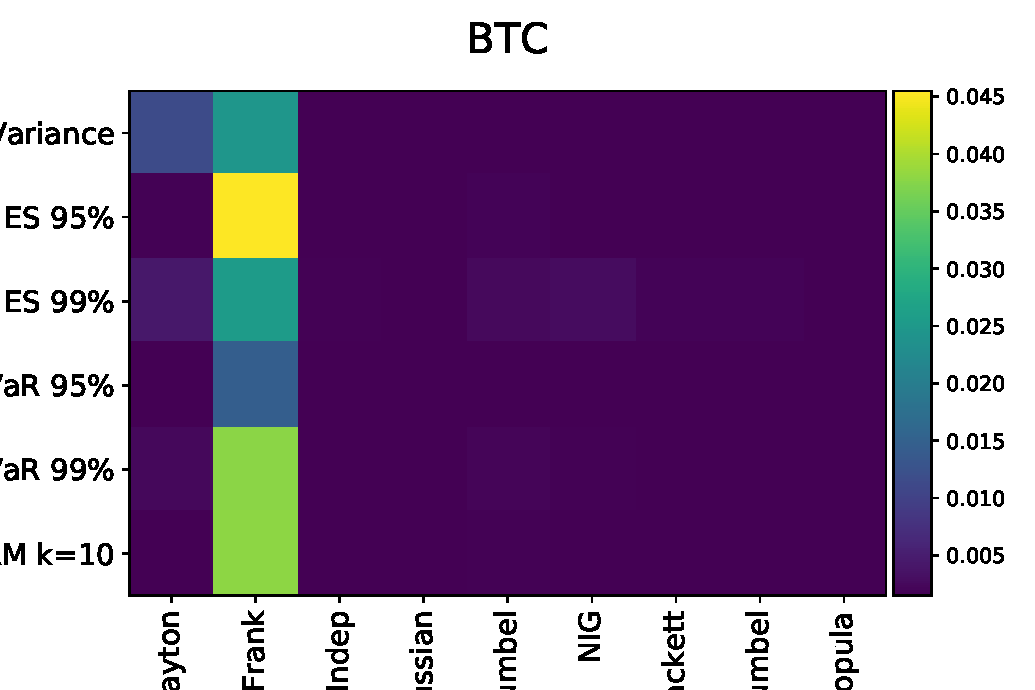
\includegraphics[width=\textwidth]{_pics/MSE_BTC.pdf}
  \caption{Mean square errors of BTC-BTCF portfolios constructed with different copula and risk minimization objectives.
    The Frank copula is inferior in the BTC-involved portfolios.
    \href{http://www.quantlet.com/}{\includegraphics[height=\baselineskip]{_pics/qletlogo_tr.png}} }
\label{fig:MSE_BTC}
\end{minipage}%
\hfill
\begin{minipage}[t]{.475\textwidth}
    \centering
    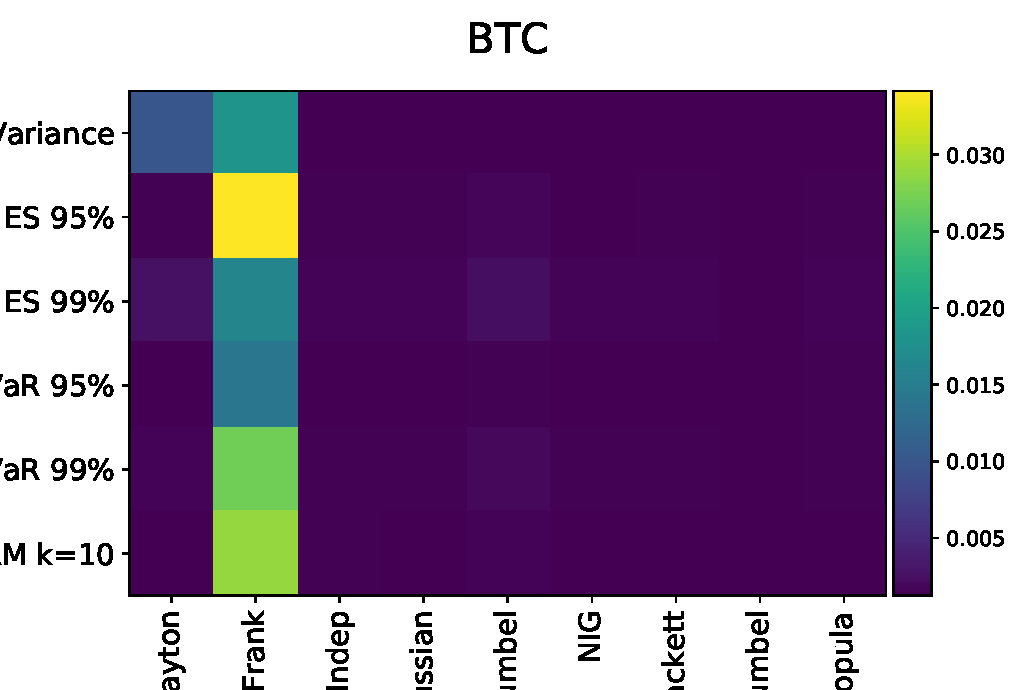
\includegraphics[width=\textwidth]{_pics/semiLowerVariance_BTC.pdf}
  \caption{Lower semivariance of BTC-BTCF portfolios constructed with different copula and risk minimization objectives.
  The Frank copula is obviously inferior.
  \href{http://www.quantlet.com/}{\includegraphics[height=\baselineskip]{_pics/qletlogo_tr.png}} }
\label{fig:SLV_BTC}
\end{minipage}
\end{figure}
\subsection{An overview of the hedged portfolios without the copula selection step}\label{subsec:HP1}
First, we analyse the results of hedged portfolios without the copula
selection step in order to get a better understanding of how a copula
affects the hedged portfolio with various risk minimization
objectives.
To do so, we inspect the hedge performance of copulas by
the mean square error and lower semi-variance.
The mean square error
is the distance between a perfect hedge and the hedged portfolio
returns $\operatorname{MSE}= \E(R^2)$.
The lower semi-variance is defined as 
$\operatorname{LSV}=\E \left( (R-\E(R))^2 \1_{\{R\leq \E(R)\}} \right)$.
All results presentedd here are out-of-sample results obtained without
the copula selection step in order to compare the performances across
copulae.

\newpage
\begin{figure}[!]
        \centering
        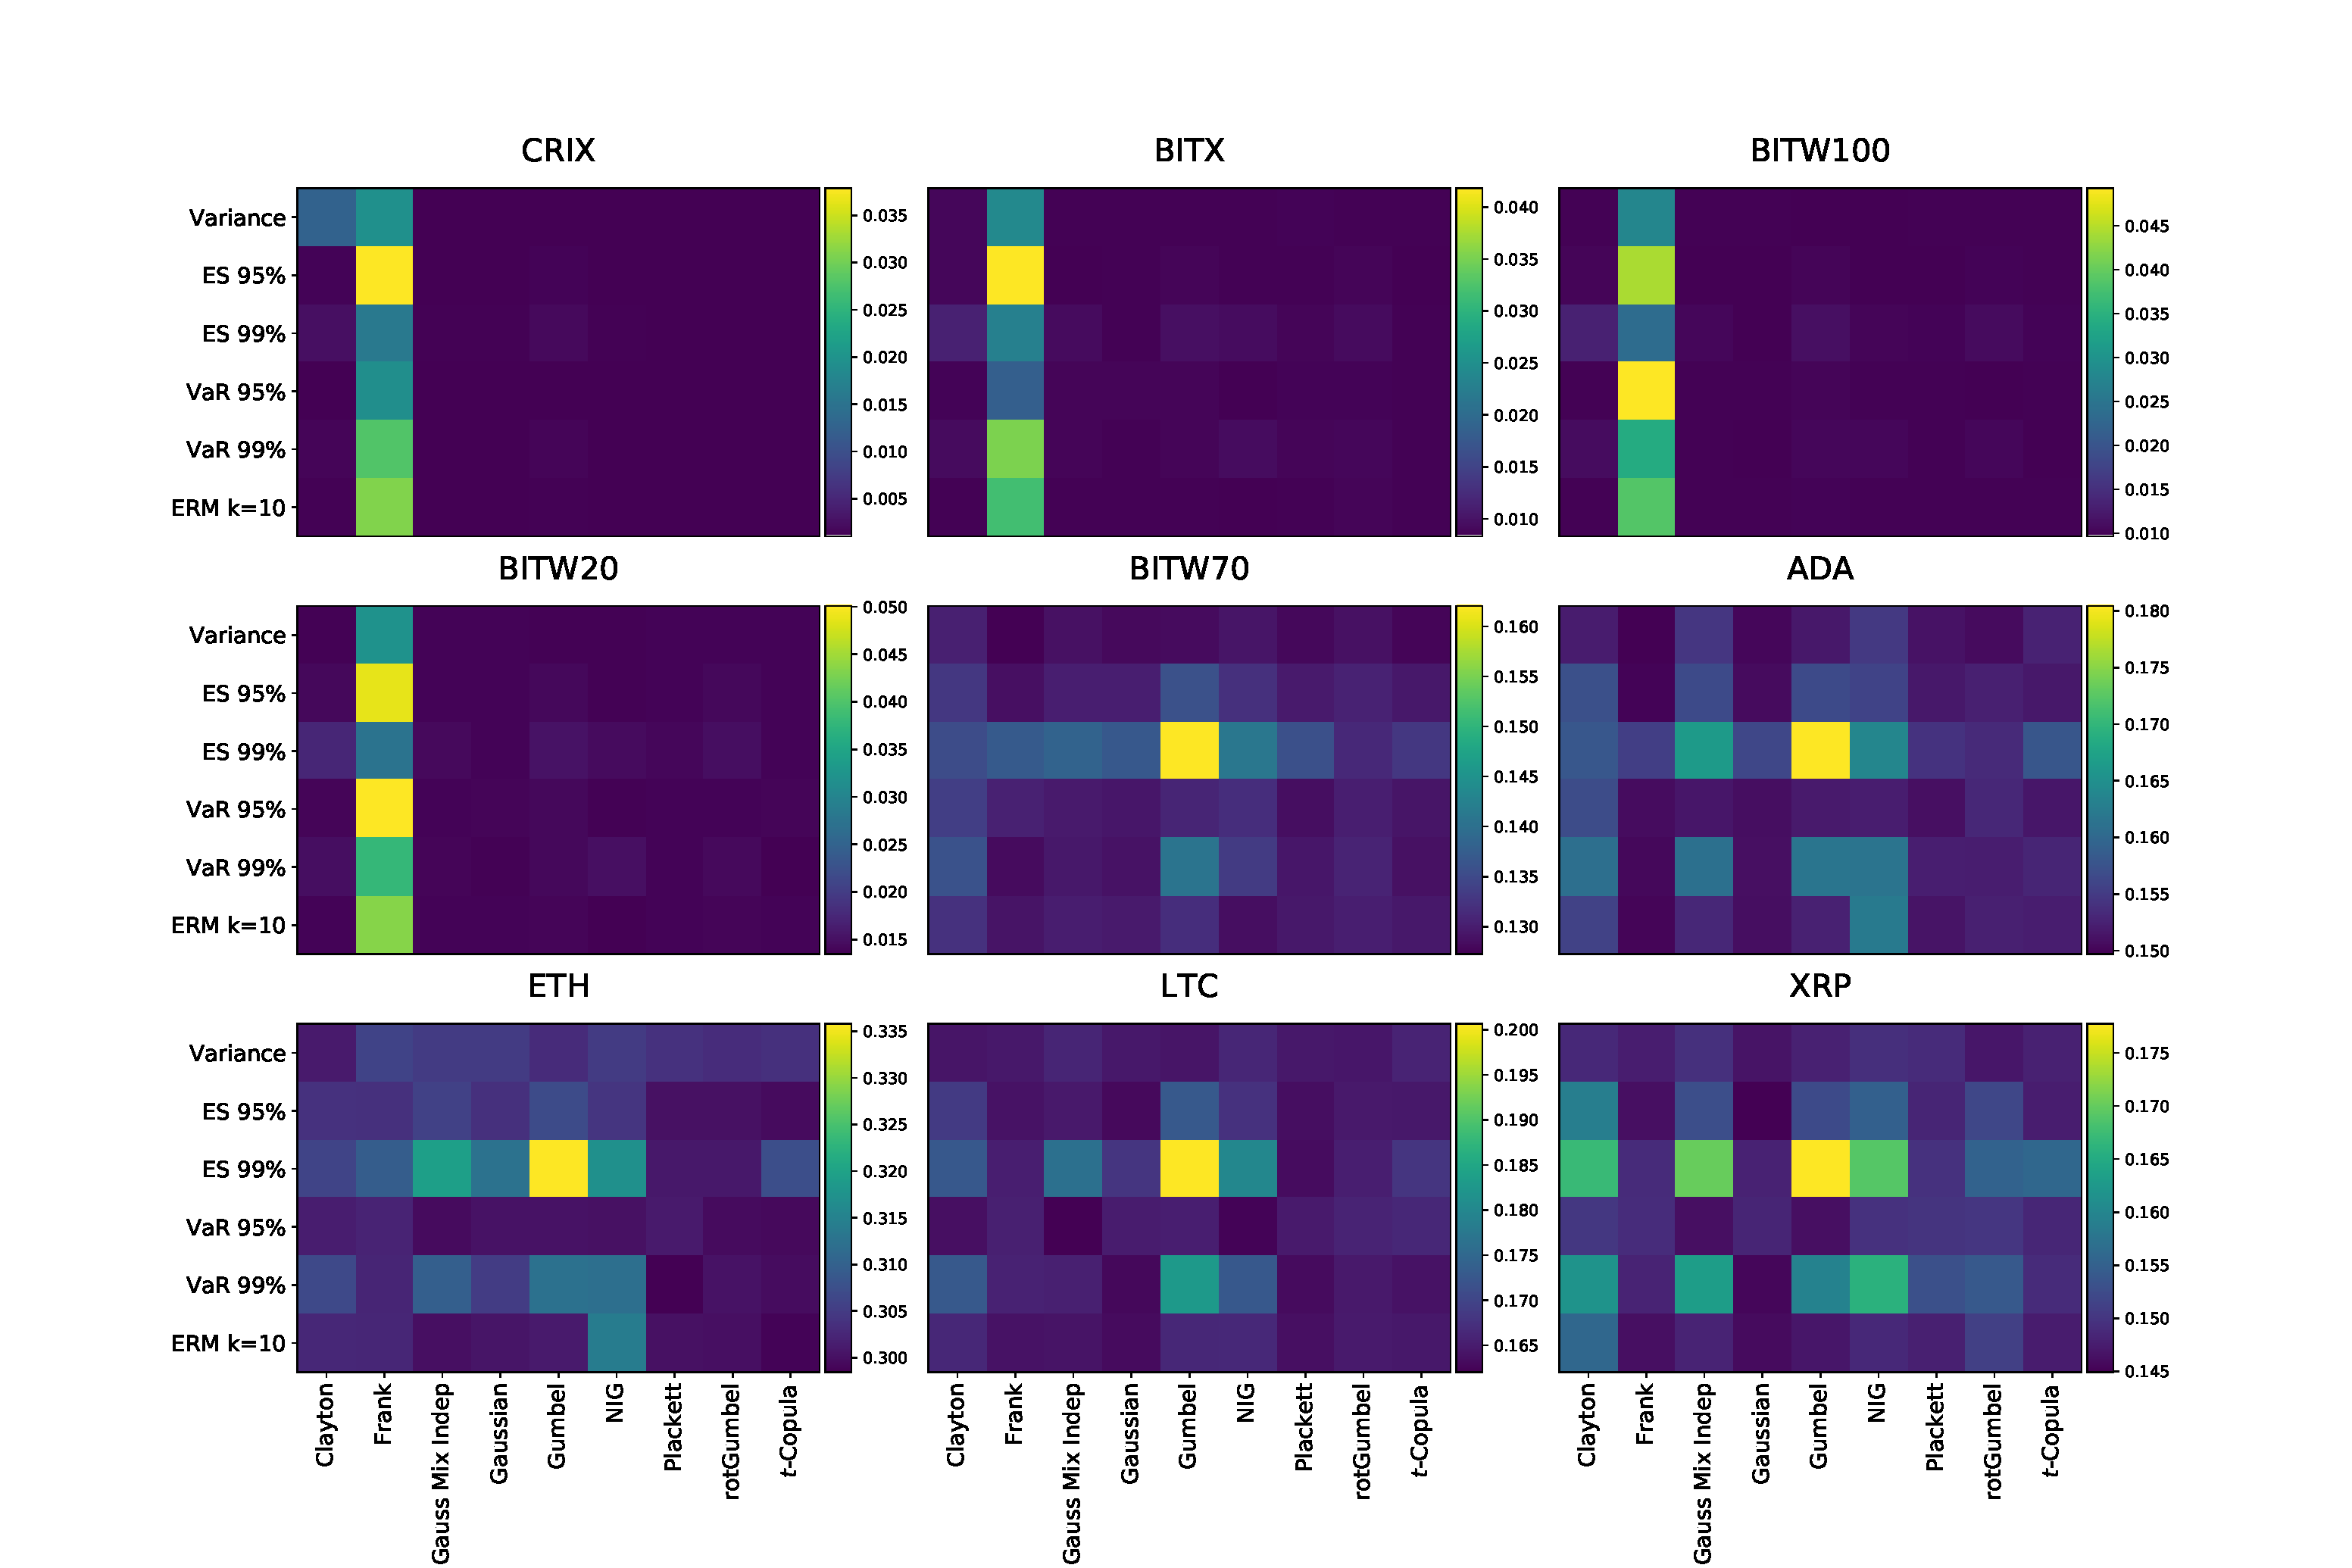
\includegraphics[width=\textwidth]{_pics/MSE_other.pdf}
      \caption{Mean square errors of portfolios constructed with different copula and risk minimization objectives.
      \href{http://www.quantlet.com/}{\includegraphics[height=\baselineskip]{_pics/qletlogo_tr.png}} }
    \label{fig:MSE_other}
%\end{subfigure}%
%\end{figure}

%\begin{figure}[!]
%\begin{subfigure}{\textwidth}\centering
        \centering
        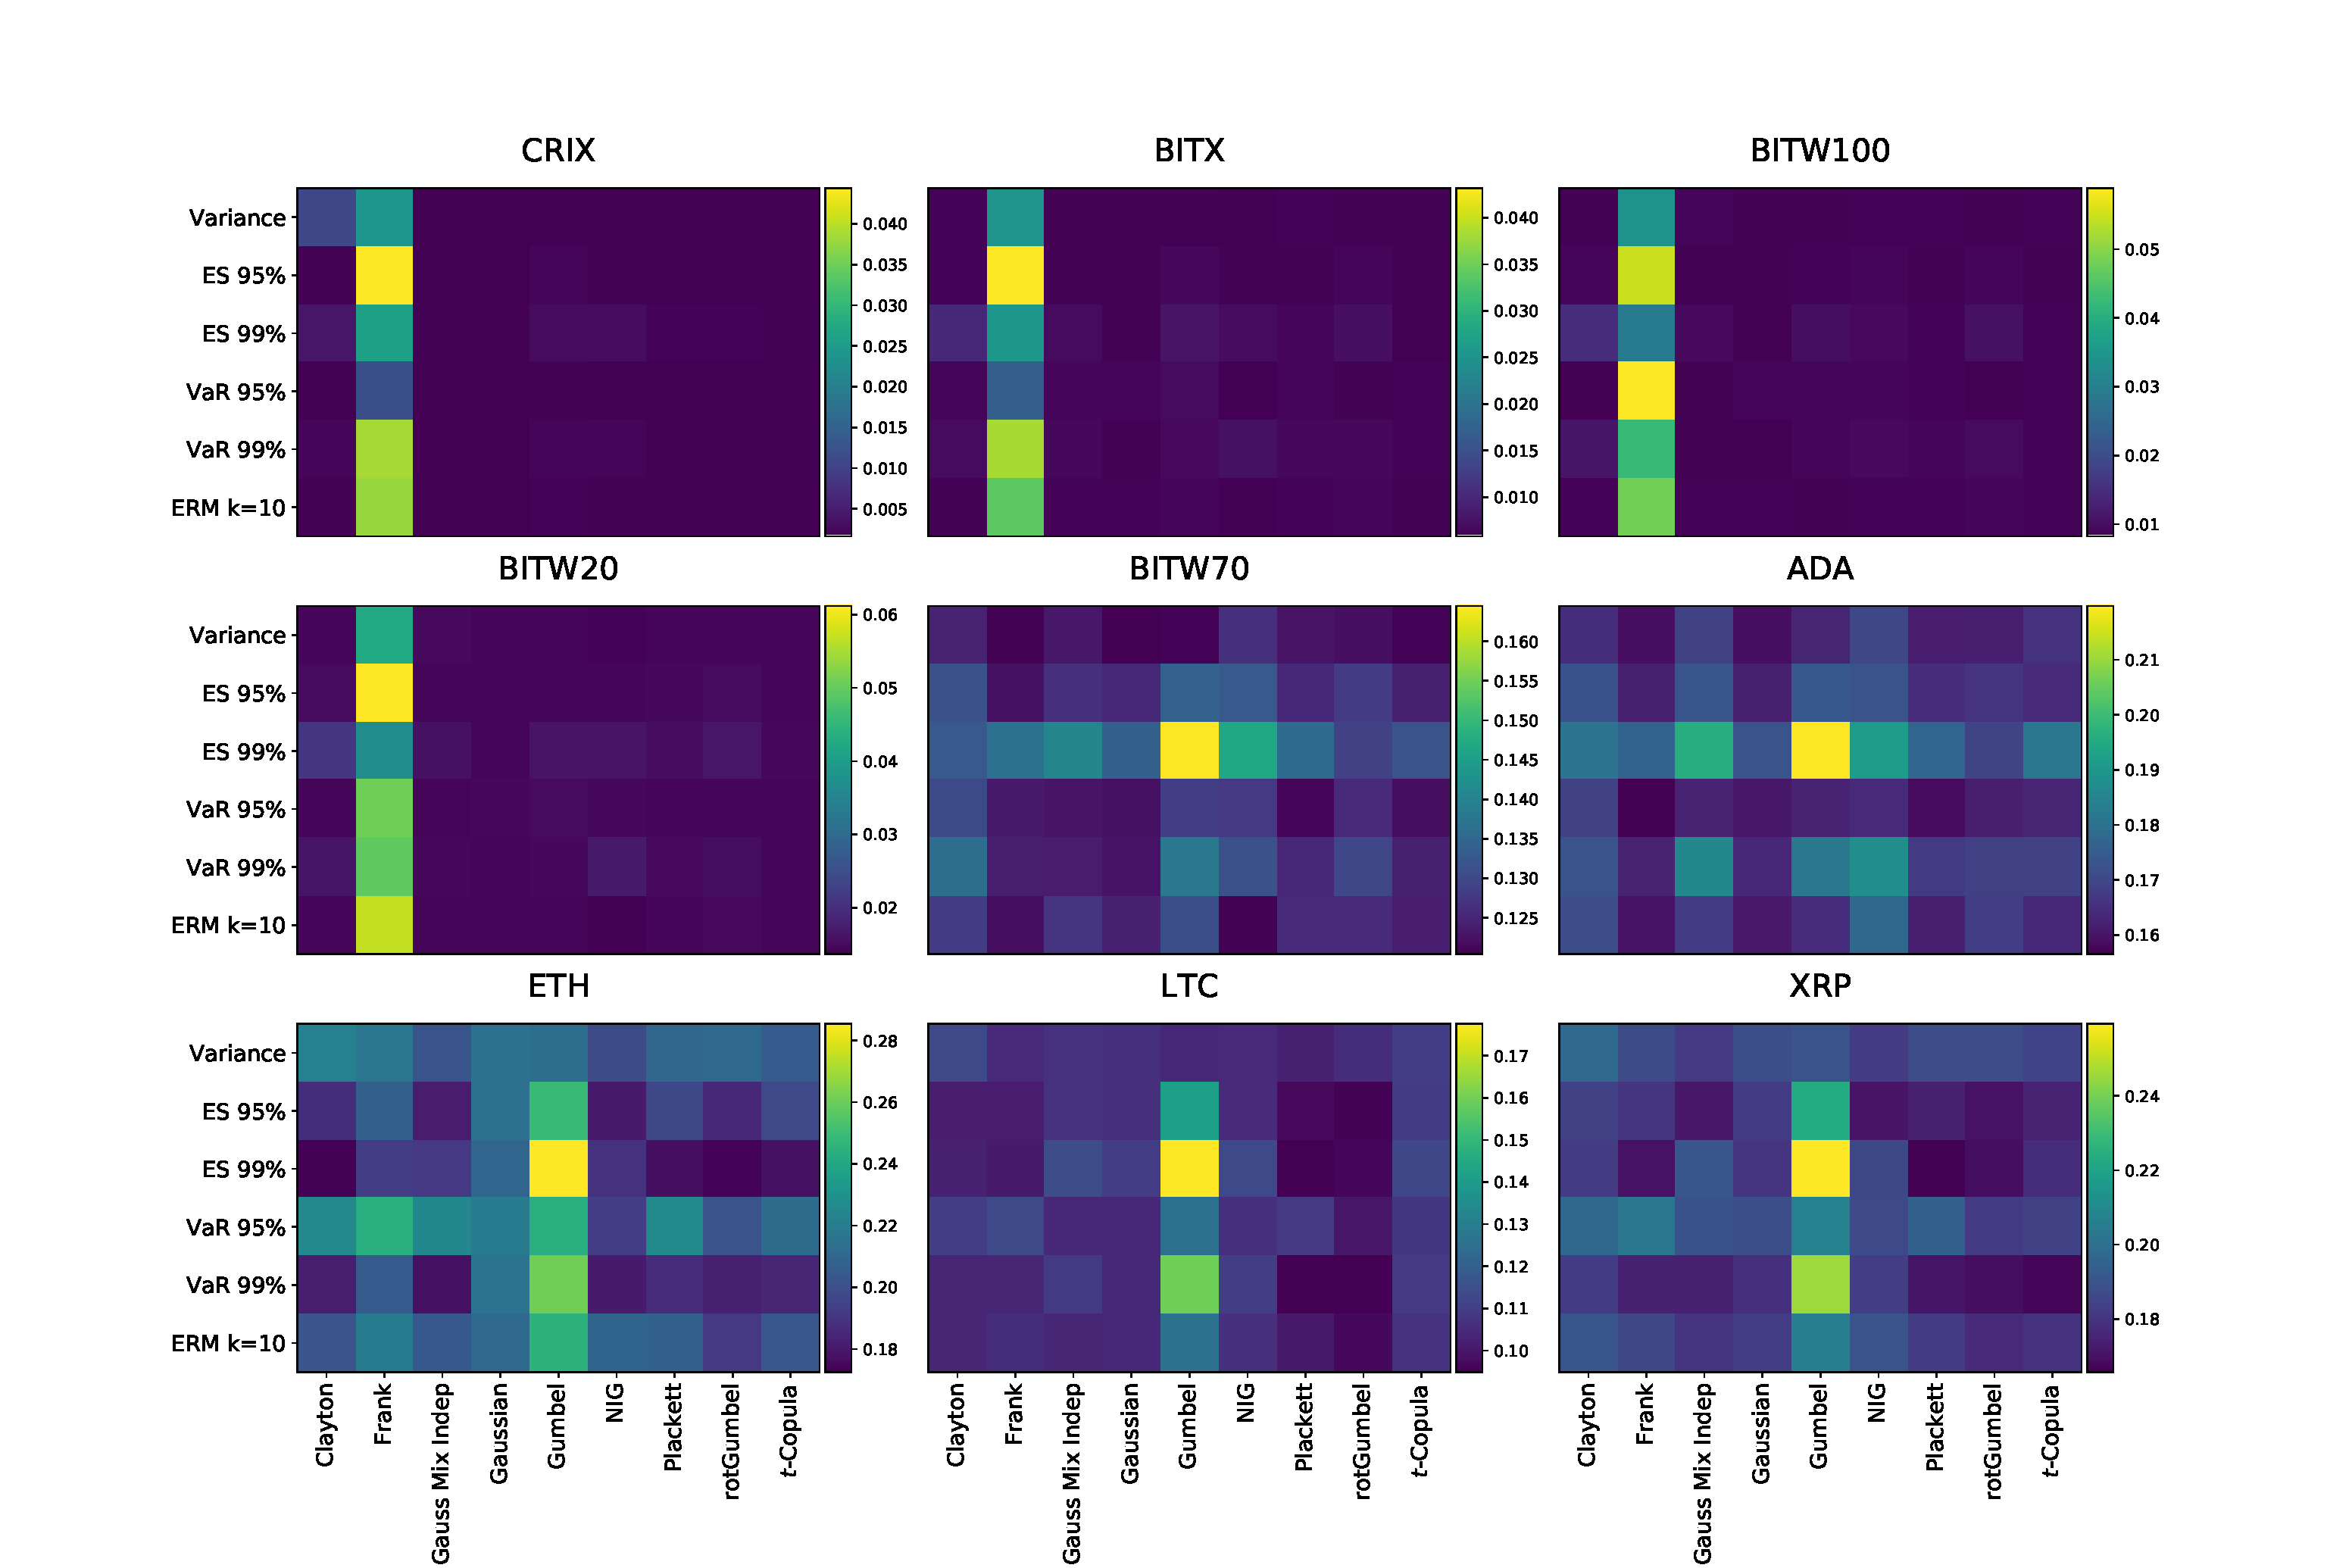
\includegraphics[width=\textwidth]{_pics/semiLowerVariance_other.pdf}
      \caption{Lower semivariance of portfolios constructed with different copula and risk minimization objectives.
%      \href{http://www.quantlet.com/}{\includegraphics[height=\baselineskip]{_pics/qletlogo_tr.png}}
  }
    \label{fig:SLV_other}
\end{figure}
\clearpage

%\textcolor{darkblue}{As presented in Fig 3 and 4, either individual cryptos or indice, their cumulative returns dropped in Mar 2020. it's due to the result of COVID19. we can explain this for these two plots.}\\
%\textcolor{darkblue}{Here i think it should insert a paragraph to interpret how you enter the copulae, otherwise it's weird that comes to Fig 5 and 6.}\\

Figure \ref{fig:MSE_BTC} and \ref{fig:SLV_BTC} are the mean square
error and lower semivariance of BTC-BTCF. We can see that the Frank copula
is the worst performing copula: 
the resulting hedged portfolio returns is far away from a perfect
hedge. \natp{\em [Can you swap the plots so that they are ordered
  according to the scales?]}
In Figures \ref{fig:MSE_other} and \ref{fig:SLV_other}, the phenomenom
of Frank copula being inferior to its counterparts can be observed
from the results of the CRIX, BITX, BITW100, and BITW20-BTCF
portfolios. 
Interestingly, the spot in those portfolios usually have a strong
dependence with the BTCF.
In contrast, the inferiority of the Frank copula is less prominent in
the BITW70, ADA, ETH, LTC and XRP-BTCF portfolios. 
We suspect that the Frank copula is not a choice to model assets with
strong dependence.

We can also observe from Figures \ref{fig:MSE_other} and
\ref{fig:SLV_other} that theGumbel copula is not performing as well as 
other copulas in the ETH, LTC, and XRP-BTCF portfolios. 
The reason is the Gumbel copula has only upper tail dependence,
while the ETH, LTC, and XRP exhibit lower tail dependence with BTCF. 
We will discuss this in the following section.

\subsection{Copula Selection Results}\label{subsec:-copula-results}
\begin{table}[t]
 \ra{1.1}
    {\begin{tabularx}{\textwidth}{lYYYYY} \toprule
         Copula/Asset & $t$ & Plackett & GMI & rotGumbel & NIG \\ \midrule
     \multicolumn{6}{l}{Individual Cryptos}                                                                                 \\
        \ \ \ BTC          & 73         & 4                 & 2                        & 1                  & 31                  \\
        \ \ \ ETH          & 3          & 6                 & 8                        & 94                 & 1                   \\
        \ \ \ ADA          & 0          & 0                 & 0                        & 0                  & 112                 \\
        \ \ \ LTC          & 13         & 0                 & 3                        & 32                 & 64                  \\
        \ \ \ XRP          & 0          & 31                & 3                        & 78                 & 0                   \\
   \multicolumn{6}{l}{Crypto Indices with BTC Constituent}                                                                  \\
        \ \ \ BITX         & 39         & 0                 & 14                       & 16                 & 12                  \\
        \ \ \ CRIX         & 47         & 0                 & 11                       & 3                  & 27                  \\
        \ \ \ BITW100      & 42         & 0                 & 8                        & 29                 & 2                   \\
    \multicolumn{6}{l}{Crypto Indices without BTC Constituent}                                                              \\
        \ \ \ BITW20       & 0          & 0                 & 0                        & 78                 & 3                   \\
        \ \ \ BITW70       & 0          & 0                 & 0                        & 80                 & 1                   \\
    \bottomrule
    \end{tabularx}
        \caption{Copula Selection Results. }









 \caption{Copula selection results (shortened).
        The values are the counts of a copula chosen by the AIC procedure during the out-of-sample period.
        Each count represents five trading days since the each testing data consists of five trading days.
        The table shows only the frequently chosen copula, i.e. $t$, Plackett, Gaussian Mix Independent (GMI), rotated Gumbel (rotGumbel), and
        Normal Inverse Gaussian factor copula (NIG).
        }
    \label{tab:copulasection}
\end{table}
Next, we inspect the copula selection result by the AIC procedure described in section~\ref{subsec:copula-selection}.
Although the copula selection is only an intermediate step to obtain the OHRs,
the result of this step can help us better understand the dependence
feature between BTCF and the assets we study in this work.
This gives us valuable information to model the assets in the future.
Decisions of the AIC procedure are summarised in Table \ref{tab:copulasection}. \medskip

Overall, the $t$-copula, rotated Gumbel (rotGumbel), and the NIG
factor copula are the most frequently chosen copulae by the AIC
procedure. \medskip

The $t$-copula is frequently chosen to model the dependence between
the BTC and BTC-involving-indices, CRIX, BITX, BITW100, and the BTC
future.
BTC and BTC-involving-indices exhibit strong (upper and lower) tail
dependence with BTCF.  We interpret tail dependence as a strong
tendency for one asset to be extreme when another is extreme and
vice versa \citep{McNeil2015}.
In fact, the $t$ copula has been recommended in various empirical
studies to model financial data, such as~\cite{zeevi2002beyond} and~
\cite{breymann2003dependence}.
Those studies suggest that the $t$-copula is a better model compared
to the Gaussian copula as financial data typically exhibit heavy tails
and tail dependence. \medskip

On the other hand, the radial symmetry of the $t$-copula appears to be
a poor choice to model the remaining hedging pairs.
\cite{demarta2005t} describe the radial symmetry feature of the $t$-copula ``strong'' as it is a radially symmetric distribution.
To be specific, if $(U_1, ..., U_d)$ is a vector distributed in $t$-copula,
then $(U_1, ..., U_d) \overset{\mathcal{L}}= (1-U_1, ...,
1-U_d)$.
This symmetry can be justified in the dependence structure between a
futures and its underlying by the theory of futures pricing,
which suggests the price of a futures is a function of the underlying
price \citep{hull2003options}.
However, there is no such relationship between a futures and an asset
which is not the underlying.
Besides, asset prices tend to crash simultaneously whereas positive development tends to be idiosyncratic. \medskip

Among the three popular copulae, rotGumbel copula shows its ability to model the dependence between ETH and BTCF.
rotGumbel also performs well when modelling dependence between XRP, BITW20, BITW70, and the BTCF.
In particular, the whole time series of the two indices, BITW20 and BITW70, are best fitted solely with the rotated Gumbel copula. \medskip

In fact, Clayton's AIC in many of the training sets is the second lowest, just higher than that of rotated Gumbel.
This is because the Clayton copula has the same ability to model the lower quantile dependence.
However, Clayton's radial like feature does not match the behaviour of
the financial data. \medskip

It is worth to mention that although the NIG factor copula is penalised heavily due to its three parameters setup,
it is frequently chosen to be the best copula to model the dependence
between individual cryptos and the BTC future.
An extreme case would be ADA, where only NIG factor is chosen in our dataset.
Another dependence structure being best described by the NIG factor
copula is the pair of LTC-BTCF, with
64 out of 112 training sets best fitted by the NIG factor copula.
Indices like BITX and CRIX are sometimes best fitted with the NIG
factor copula as well, accounting for modelling 12 and 27 training
sets respectively.
The popularity of the NIG factor copula reflects the ability of the copula to
model very complex dependence structure: the
NIG factor copula is able to model the tail, radial asymmetry, and
off-diagonal (the region away from the diagonal line $(0,0)$ to
$(1,1)$, see figure \ref{fig:copulaeScatterPlot}) behaviour. \natp{\em
  [I think you did not understand my comment. It is clear what the
  ``off-diagonal'' is. It is unclear what is meant by ``off-diagonal
  behaviour''. Do you mean extremes on the other diagonal? Do you mean
  a cloud of points away from the diagonal? Not sure what the NIG
  factor copula is capable of modelling in this respect. Perhaps you
  have a reference?]}
  


The Frank copula is generally not a good choice to model financial
data (as also reported by \cite{barbi2014copula}).
Plackett is characterised by its dependence parameter being equal to
the cross-product ratio % \citep{joe1997multivariate}
. \natp{\em [Provide
  reference to Equation (32).]}
However, apparently, this property does not capture the dependence
structure of cryptos and BTCF.


\subsection{Hedged portfolios with the copula selection step}\label{subsec:HP2}
%\begin{table}[t] \centering
%    %\begin{table}[!] \centering
\resizebox{.75\textwidth}{!}{%
\begin{tabular}{lcccccc}
\toprule
{} &    Mean \% &      Std \% &    Skew &    Kurt &       MD \% & Date of MD\\
\midrule
Variance &  0.0215 &  0.3221 & -1.0119 &  3.1929 & -0.0144 &  2020-11-30 \\
VaR 95\%  &  0.0253 &  0.3294 & -0.9725 &  3.4373 & -0.0153 &  2020-11-30 \\
VaR 99\%  &  0.0176 &  0.3270 & -1.0405 &  3.3742 & -0.0157 &  2020-11-30 \\
ES 95\%   &  0.0204 &  0.3234 & -1.0150 &  3.4423 & -0.0156 &  2020-11-30 \\
ES 99\%   &  0.0148 &  0.3476 & -0.8354 &  3.3054 & -0.0162 &  2020-11-30 \\
ERM k=10 &  0.0223 &  0.3221 & -1.0008 &  3.4153 & -0.0152 &  2020-11-30 \\
\bottomrule
\end{tabular}}
\caption{Summary statistics of BTC-BTCF hedge portfolios out-of-sample daily returns under different risk minimisation objectives.}
\label{tab:BTCrh}
%\end{table}
%    \caption{Summary statistics of BTC-BTCF hedge portfolios out-of-sample daily returns under different risk minimisation objectives.}
%\label{tab:BTCrh}
%\end{table}
\begin{landscape}
  \begin{table}[!] \centering
\resizebox{.8\paperheight}{!}{%
\begin{tabular}{l*{10}{r}}
\toprule
{} &   BTC & ETH & ADA & LTC & XRP & BITX & CRIX & BITW100 & BITW20 & BITW70\\
\midrule
  \multicolumn{10}{l}{Spots assets only}   \\
\ \ \ Mean \%  &      0.3915 &      0.6819 &      0.9467 &      0.3227 &      0.2987 &      0.4308 &      0.4602 &      0.4683 &      0.6249 &      0.6353 \\
\ \ \ Std \%   &      4.4023 &      6.0103 &       6.699 &      6.4781 &      7.9843 &      4.5676 &       4.542 &      4.6174 &      5.5021 &      5.8155 \\
\ \ \ MD \%    &    -25.9965 &    -32.0144 &    -26.8528 &    -37.5913 &    -52.7652 &     -27.022 &    -27.1385 &    -27.2694 &    -31.0092 &    -32.3453 \\
\ \ \ MD date &  2020-03-12 &  2020-03-12 &  2020-03-12 &  2021-05-19 &  2020-12-23 &  2020-03-12 &  2020-03-12 &  2020-03-12 &  2020-03-12 &  2021-05-19 \\
  \multicolumn{10}{l}{Variance minimizing portfolios}   \\
\ \ \ Mean \%  &      0.0215 &      0.2823 &      0.5617 &     -0.0871 &     -0.0123 &      0.0561 &      0.0812 &      0.0855 &      0.2429 &      0.2706 \\
\ \ \ Std \%   &      0.3221 &      3.8741 &      5.2722 &      3.9052 &      7.1537 &      0.9954 &      0.9183 &      1.1986 &      3.5846 &      3.8838 \\
\ \ \ MD \%    &     -1.4393 &    -17.7421 &    -13.8687 &    -28.3029 &    -52.5236 &     -7.7567 &     -7.1025 &    -11.3866 &     -21.468 &    -23.9984 \\
\ \ \ MD date &  2020-11-30 &  2021-05-19 &  2021-01-08 &  2021-05-19 &  2020-12-23 &  2021-05-19 &  2021-05-19 &  2021-05-19 &  2021-05-19 &  2021-05-19 \\
  \multicolumn{10}{l}{VaR 95\% minimizing portfolios}   \\
\ \ \ Mean \%  &      0.0253 &      0.3084 &      0.5726 &     -0.0742 &      0.0208 &      0.0562 &      0.0863 &      0.0846 &      0.2728 &      0.2847 \\
\ \ \ Std \%   &      0.3294 &      3.8944 &      5.2204 &      3.9145 &       7.152 &       0.993 &      0.9151 &       1.198 &       3.594 &      3.9133 \\
\ \ \ MD \%    &     -1.5347 &     -19.175 &    -14.6974 &    -28.3672 &    -52.5667 &     -7.5639 &     -6.9744 &    -11.2582 &    -22.0733 &    -24.6513 \\
\ \ \ MD date &  2020-11-30 &  2021-05-19 &  2021-05-19 &  2021-05-19 &  2020-12-23 &  2021-05-19 &  2021-05-19 &  2021-05-19 &  2021-05-19 &  2021-05-19 \\
  \multicolumn{10}{l}{VaR 99\% minimizing portfolios}   \\
\ \ \ Mean \%  &      0.0176 &      0.2977 &      0.5562 &     -0.0852 &      0.0352 &      0.0593 &      0.0738 &      0.0823 &      0.2499 &      0.2788 \\
\ \ \ Std \%   &       0.327 &      3.9132 &      5.3466 &      4.1503 &      7.1658 &      1.0178 &      0.9695 &      1.2338 &       3.621 &      3.9257 \\
\ \ \ MD \%    &     -1.5689 &    -18.6061 &    -15.4795 &    -29.0915 &    -52.5727 &     -8.0299 &     -7.0185 &    -11.8752 &    -21.6634 &    -24.5294 \\
\ \ \ MD date &  2020-11-30 &  2021-05-19 &  2021-05-19 &  2021-05-19 &  2020-12-23 &  2021-05-19 &  2021-05-19 &  2021-05-19 &  2021-05-19 &  2021-05-19 \\
  \multicolumn{10}{l}{ES 95\% minimizing portfolios}   \\
\ \ \ Mean \%  &      0.0204 &      0.3082 &      0.5525 &     -0.0808 &      0.0176 &      0.0591 &      0.0777 &      0.0848 &      0.2608 &      0.2785 \\
\ \ \ Std \%   &      0.3234 &       3.889 &      5.2673 &      3.9829 &      7.1533 &      1.0065 &      0.9207 &      1.2125 &      3.6115 &      3.9157 \\
\ \ \ MD \%    &     -1.5629 &    -18.7819 &    -14.9647 &    -28.4608 &    -52.5698 &     -7.6211 &     -6.9894 &    -11.1357 &     -21.543 &    -24.3474 \\
\ \ \ MD date &  2020-11-30 &  2021-05-19 &  2021-05-19 &  2021-05-19 &  2020-12-23 &  2021-05-19 &  2021-05-19 &  2021-05-19 &  2021-05-19 &  2021-05-19 \\
  \multicolumn{10}{l}{ES 99\% minimizing portfolios}   \\
\ \ \ Mean \%  &      0.0148 &       0.308 &      0.5016 &     -0.1029 &       -0.02 &      0.0598 &      0.0835 &      0.0781 &      0.2538 &       0.266 \\
\ \ \ Std \%   &      0.3476 &      3.8954 &       5.404 &      4.1581 &      7.2887 &      1.0312 &      0.9461 &       1.264 &      3.6323 &       3.932 \\
\ \ \ MD \%    &     -1.6225 &    -18.7625 &    -15.4481 &    -29.1727 &      -52.57 &     -7.7424 &     -7.0203 &    -11.9263 &    -21.9866 &    -24.4764 \\
\ \ \ MD date &  2020-11-30 &  2021-05-19 &  2021-05-19 &  2021-05-19 &  2020-12-23 &  2021-05-19 &  2021-05-19 &  2021-05-19 &  2021-05-19 &  2021-05-19 \\
  \multicolumn{10}{l}{ERM $k=10$ minimizing portfolios}   \\
\ \ \ Mean \%  &      0.0223 &      0.3117 &      0.5722 &     -0.0512 &      0.0155 &       0.059 &       0.084 &      0.0853 &      0.2564 &      0.2818 \\
\ \ \ Std \%   &      0.3221 &      3.8679 &       5.359 &      3.8812 &      7.1579 &      1.0078 &      0.9087 &      1.2032 &      3.6009 &      3.9074 \\
\ \ \ MD \%    &     -1.5242 &    -18.8729 &    -14.3885 &    -28.0879 &    -52.5689 &     -7.8581 &      -7.053 &    -11.1846 &     -21.592 &     -24.525 \\
\ \ \ MD date &  2020-11-30 &  2021-05-19 &  2021-01-08 &  2021-05-19 &  2020-12-23 &  2021-05-19 &  2021-05-19 &  2021-05-19 &  2021-05-19 &  2021-05-19 \\
\bottomrule
\end{tabular}}
\end{table}
  \end{landscape}
Table~\ref{tab:bigTable} presents the first two moments, maximum drawdown (MD) and the date of MD of the hedge portfolios.
We observe that the statistics of the portfolios with different objectives are similar to each other.
We provide the detail in Tables~\ref{tab:var_rh} to \ref{tab:ERM_rh} in the appendix.

%For the other spots \natp{\em [Do you mean cryptocurrencies? Or all
%  hedges? Then maybe use the word ``instruments to be hedged'' or ``instruments''.]}, tables~\ref{tab:var_rh} to table~\ref{tab:ERM_rh} summarise the statistics
%of daily returns of hedged portfolios.  \natp{\em [Table and Figure if
%  you reference them directly.]} \natp{\em [Why are the tables
%  oversized? Bring them down to normal size.]} \natp{\em [Also, think
%  carefully what VaR 5\% means. If you are taking the 5\% quantile of
%  P\&L data, then it's VaR 95\%.]}
%The tables look repeating so we place them in the appendix. \natp{\em
%  [I suggest to throw out skewness and kurtosis and place everything in one
%  table, landscape. Otherwise, the reader will need to scroll back and
%  forth in order to compare (or decide to just ignore the tables).]}
%This is because the optimal hedge ratios of different risk minimization objectives fall into a small range. \medskip

Unsurprisingly, the BTC-involved spots, i.e. BTC, CRIX, BITX, and BITW100, are well hedged by the BTCF regardless of risk minimization objective.
Contrarily, BTC-not-involved spots' portfolios are less promising.
Those hedge portfolios' returns are as volatile as the assets, see for example ADA and XRP.
We will further discuss the effectiveness of hedge in the next section. %\ref{sec: HE results}.

\subsection{Hedging Effectiveness Results}\label{sec: HE results}
\begin{figure}[t]
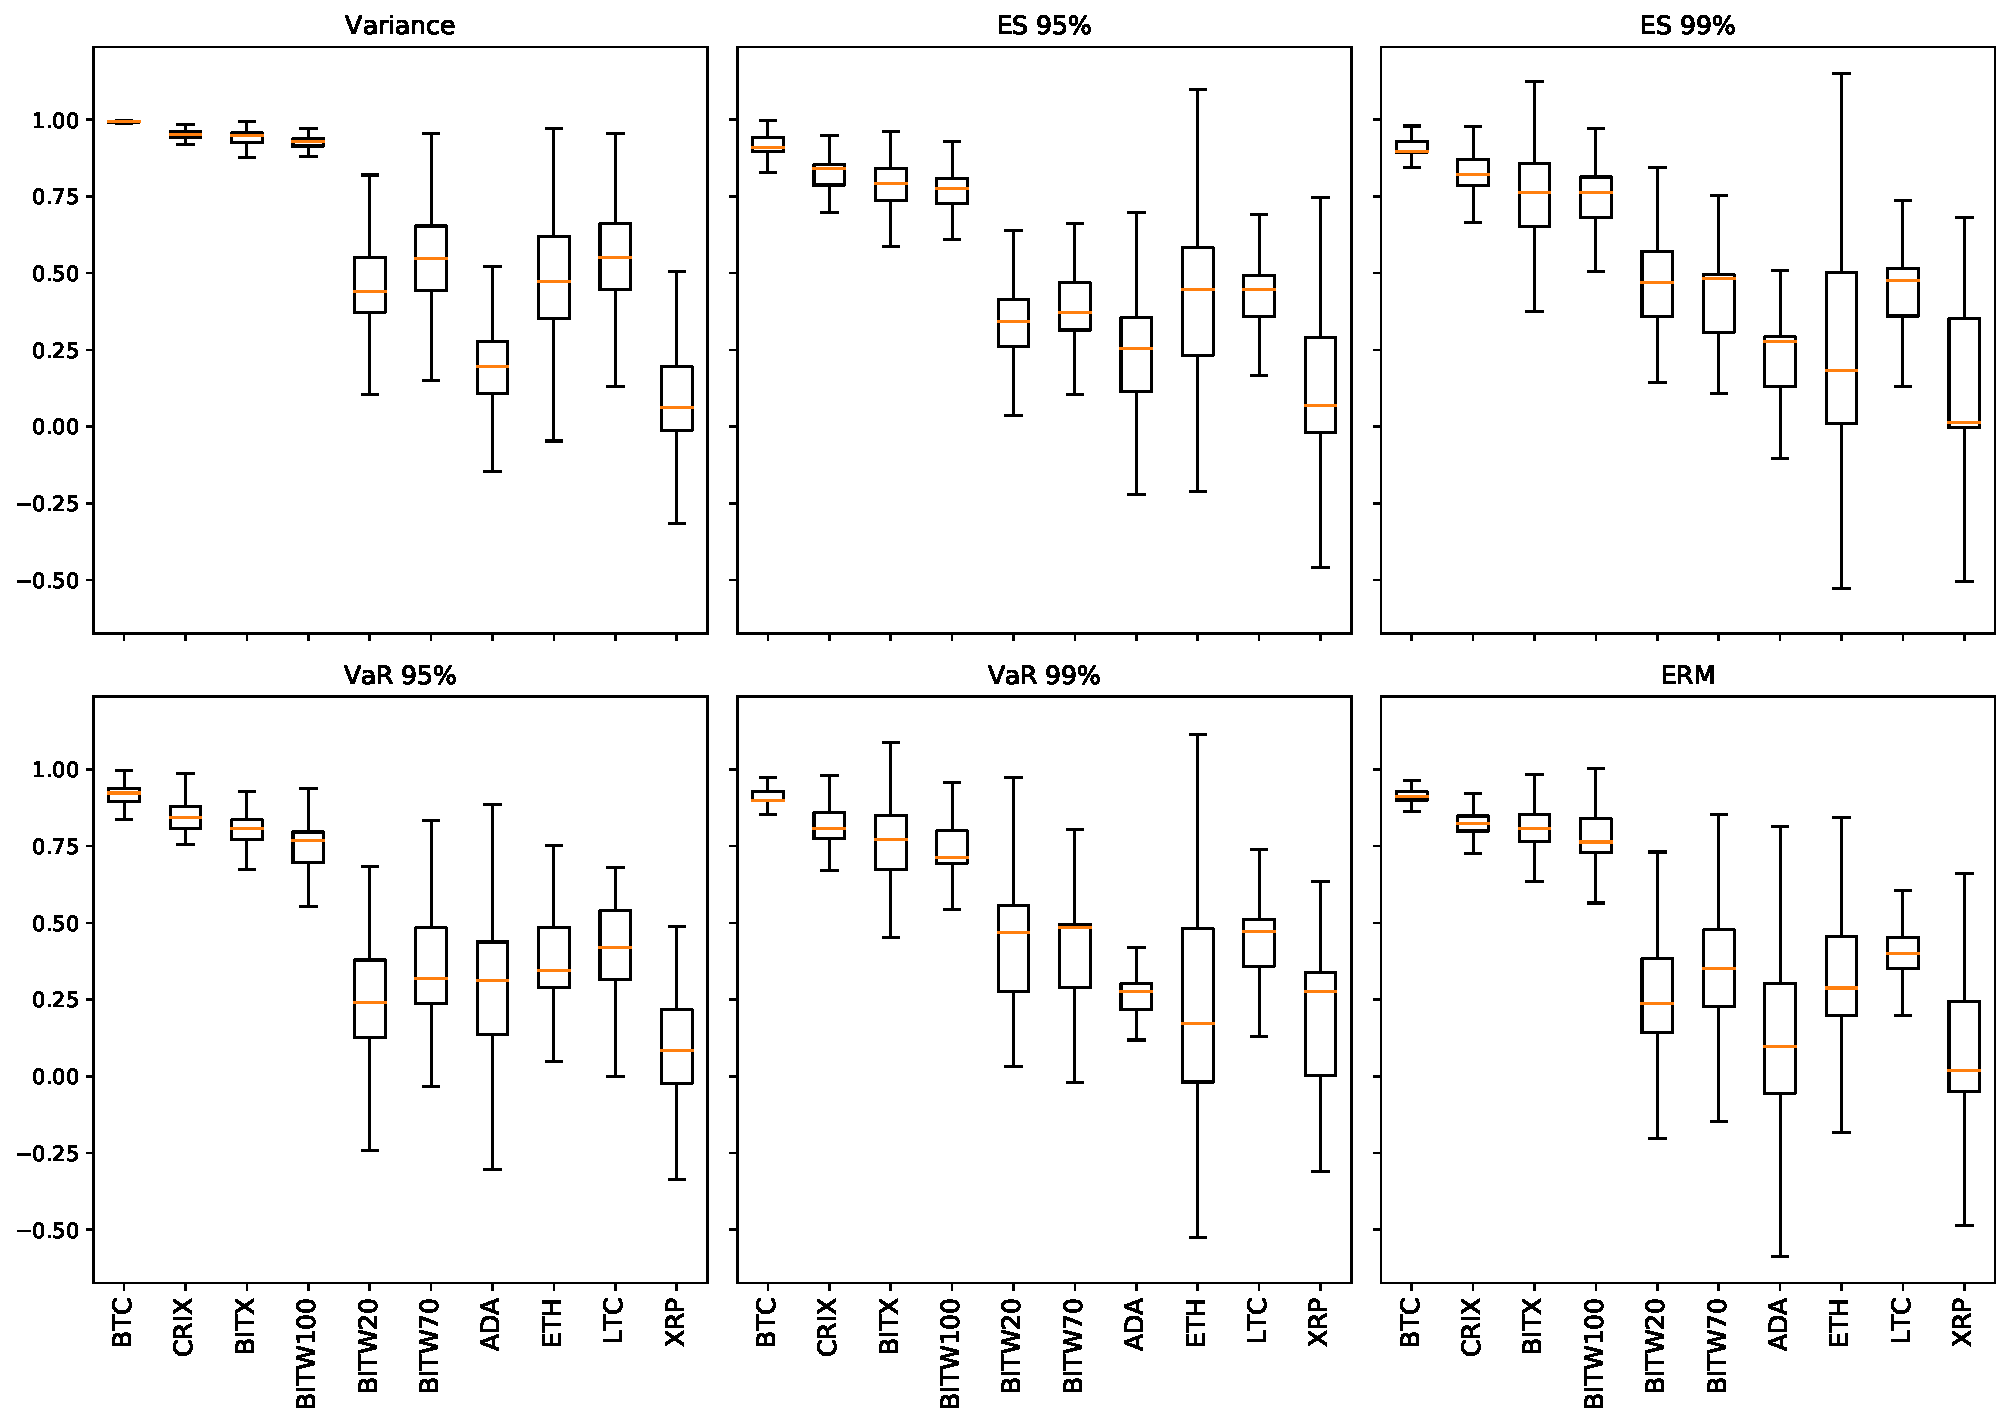
\includegraphics[width=\textwidth]{_pics/ES5_HE_boxplot.pdf}
  \caption{Hedging effectiveness (HE) of portfolios with different risk minimization objectives evaluated by the corresponding risk minimization objectives.
            The boxplots indicate the the median, upper quartile, lower quartile, minimium and maximum of the bootstrapped HE.
            The HE of BTC-involved spots are significantly higher than that of BTC-not-involved spots.
  \href{http://www.quantlet.com/}{\includegraphics[height=\baselineskip]{_pics/qletlogo_tr.png}} }
\label{fig:HEboxplot}
\end{figure}
In this section, we analyse the out-of-sample hedging effectiveness (HE) of BTCF as hedging.
HE is defined as $$\text{HE} = 1-\frac{\rho_h}{\rho_s},$$
a measure of the percentage reduction of portfolio risk attribute, in our case the spot $\rho_s$,
to hedged portfolio risk attribute $\rho_h$.
A higher HE indicates a greater risk reduction and thus the hedge is more effective. \medskip

The HE above is a generalisation of how \citet{ederington1979hedging} evaluate hedging performance.
In addition to variance, we include the risk measures which act as loss function while searching for OHR: ES 95\% and 99\%, VaR 95\% and 99\% and ERM. \medskip

The formulation above gives a point estimate per testing data.
However, each of our test data contain only 5 data points, the length is not sufficient to draw meaningful risk measure results.
To address this issue, we apply bootstrapping method on the concatenated test data time series as described in the beginning of the result section. \medskip

The bootstrapping method is known to be a powerful nonparametric tool for approximating complicated statistics~\citep{efron1994introduction, davison1997bootstrap}.
We apply stationary block bootstrapping to the time series introduced by \cite{Politis1994} in our analysis in order to preserve the temporal structure of the data while sampling.
The configuration of stationary bootstrapping procedure in this work is as follows.
Assume a time series with $N$ observations $\{X_t\}_{t \in [1,N]}$ is a strong stationary, weakly dependence time series of interest,
we form blocks of samples $B = \{X_i, ..., X_{i+j-1}\}$.
Index $i$ is a random variable uniformly distributed over
$[1,2,...,N]$ and $j$ is geometric distributed random variable with parameter $p$.
The block index $i$ and block length $j$ are independent.
For any index $k$ which is greater than $N$, the sample $X_k$ is defined to be $X_{k(\mod N)}$.
For each block, we calculate the hedging effectiveness with different risk measures mentioned above.
We choose $p=1/250$, implying the average block length is 250.
This average block length is chosen to reasonably calculate ES and VaR.
100 blocks are drawn for each risk minimising objective and
spot. \medskip
%\natp{\em [You need to go over this again. There are many
%  grammatical errors in there that need to be fixed. Also explain that
%  expected block length is 200 so that ES99\% and VaR99\% can be
%  calculated. Is the hedge ratio calculated for each sample drawn,
%  etc.? ]}

Figure \ref{fig:HEboxplot} report the bootstrapped HE samples from the concatenated out-of-sample hedge portfolio return.
As expected, the BTC involving spots, the BTC, CRIX, BITX and BITW100, are well hedged by the BTCF.
The HEs of BTCF to other cryptos and indices are substantially lower than to the BTC involving spots, but the consistency the performances across different risk reduction objectives and HE evaluation remains.
%\natp{\em[It does not
%  make sense to compare across different risk measures, so I suggest
%  to delete the last statement. }

%\natp{[How can HE be negative??? Especially
%  for variance this is impossible.]}

\natp{\em [We need some proper conclusions here.
  \begin{itemize}
  \item It is noticable that the HE of variance is highest.
  \item Comparing ES95\% and ES99\%, it is seen that ES95\%
    performs better. This is an indication that tail risk remmains
    despite hedging. 
  \end{itemize}
  ]}

\natp{\em [A general conclusion is needed. That ES95\% / Var95\%
  perform better than their 99\% counterparts is also evident from
  Figures 7 and 8. So focussing on tail risk by choosing an extreme tail risk
  measure does not lead to a promising hedge. Also variance performs
  well, especially for the lower correlated instruments /
  indices. Var95\% also performs well across all copulas. Please check
  if the tables in the appendix confirm this.\\
  Main conclusion is that the choice of copula highlights the 
  differences in the instruments / indices and their relationships
  with the futures contract. Unfortunately, we see that the copula
  choice does not always lead to the best hedge (see e.g.\ ADA), where
  Frank, Gaussian, Plackett and rotGumbel perform much better in
  terms of MSE. I suspect that has to do with the fact that hedging is
  necessarily linear, so a better copula model may not necessarily
  attain a better (linear) hedge. This means that the copula selection
  results should be taken as interesting by themselves. Also, they
  might be useful if using more than one hedge instrument, e.g.\ by
  including options as hedge instruments.]}



%%% Local Variables:
%%% mode: latex
%%% TeX-master: "SRM"
%%% End:
